% Copyright (c) 2022 by Lars Spreng
% This work is licensed under the Creative Commons Attribution 4.0 International License. 
% To view a copy of this license, visit http://creativecommons.org/licenses/by/4.0/ or send a letter to Creative Commons, PO Box 1866, Mountain View, CA 94042, USA.

%~~~~~~~~~~~~~~~~~~~~~~~~~~~~~~~~~~~~~~~~~~~~~~~~~~~~~~~~~~~~~~~~~~~~~~~~~~~~~~
% You can add your packages and commands to the loadslides.tex file. 
% The files in the folder "styles" can be modified to change the layout and design of your slides.
% I have included examples on how to use the template below. 
% Some of it these examples are taken from the Metropolis template.
%~~~~~~~~~~~~~~~~~~~~~~~~~~~~~~~~~~~~~~~~~~~~~~~~~~~~~~~~~~~~~~~~~~~~~~~~~~~~~~


\documentclass[
11pt,notheorems,compress,hyperref={pdfauthor=Maghfira Ramadhani}
]{beamer}


% Copyright (c) 2022 by Lars Spreng
% This work is licensed under the Creative Commons Attribution 4.0 International License. 
% To view a copy of this license, visit http://creativecommons.org/licenses/by/4.0/ or send a letter to Creative Commons, PO Box 1866, Mountain View, CA 94042, USA.

%~~~~~~~~~~~~~~~~~~~~~~~~~~~~~~~~~~~~~~~~~~~~~~~~~~~~~~~~~~~~~~~~~~~~~~~~~~~~~~
% Add your packages and commands to this file
%~~~~~~~~~~~~~~~~~~~~~~~~~~~~~~~~~~~~~~~~~~~~~~~~~~~~~~~~~~~~~~~~~~~~~~~~~~~~~~

%~~~~~~~~~~~~~~~~~~~~~~~~~~~~~~~~~~~~~~~~~~~~~~~~~~~~~~~~~~~~~~~~~~~~~~~~~~~~~~
\RequirePackage{palatino}
\RequirePackage[utf8]{inputenc}
\RequirePackage[T1]{fontenc}

\usefonttheme{serif}

\usepackage{styles/elegantmacros}
\usefolder{styles}
\usetheme[style=blue]{elegant}

\newcommand{\makepart}[1]{ % For convenience
\part{#1} \frame{\partpage}
}

%~~~~~~~~~~~~~~~~~~~~~~~~~~~~~~~~~~~~~~~~~~~~~~~~~~~~~~~~~~~~~~~~~~~~~~~~~~~~~~

%~~~~~~~~~~~~~~~~~~~~~~~~~~~~~~~~~~~~~~~~~~~~~~~~~~~~~~~~~~~~~~~~~~~~~~~~~~~~~~
% Figures
\RequirePackage{booktabs}
\RequirePackage{colortbl}
\RequirePackage{ragged2e}
\RequirePackage{schemabloc}
%\RequirePackage{natbib}
\RequirePackage{caption}
\RequirePackage{subcaption}
\RequirePackage{tabularx}
\RequirePackage{array}
\RequirePackage{multirow}
\usepackage[
  style=authoryear, 
]{biblatex}
\addbibresource{references.bib}
\newcolumntype{Y}{>{\centering\arraybackslash}X}

%~~~~~~~~~~~~~~~~~~~~~~~~~~~~~~~~~~~~~~~~~~~~~~~~~~~~~~~~~~~~~~~~~~~~~~~~~~~~~~

%~~~~~~~~~~~~~~~~~~~~~~~~~~~~~~~~~~~~~~~~~~~~~~~~~~~~~~~~~~~~~~~~~~~~~~~~~~~~~~
% Figures
\RequirePackage{wrapfig}
\RequirePackage{pgfplots}
\RequirePackage{graphicx}
\RequirePackage{adjustbox}
\RequirePackage{environ}
\pgfplotsset{compat=1.18}

\makeatletter
\newsavebox{\measure@tikzpicture}
\NewEnviron{scaletikzpicturetowidth}[1]{%
  \def\tikz@width{#1}%
  \def\tikzscale{1}\begin{lrbox}{\measure@tikzpicture}%
  \BODY
  \end{lrbox}%
  \pgfmathparse{#1/\wd\measure@tikzpicture}%
  \edef\tikzscale{\pgfmathresult}%
  \BODY
}
\makeatother
%~~~~~~~~~~~~~~~~~~~~~~~~~~~~~~~~~~~~~~~~~~~~~~~~~~~~~~~~~~~~~~~~~~~~~~~~~~~~~~

%~~~~~~~~~~~~~~~~~~~~~~~~~~~~~~~~~~~~~~~~~~~~~~~~~~~~~~~~~~~~~~~~~~~~~~~~~~~~~~
% Maths 
\RequirePackage{textcomp}
\RequirePackage{amsmath} 
\RequirePackage{amsthm}
\RequirePackage{mathtools}
%\RequirePackage{bbm}
%\RequirePackage{algorithm}
%\RequirePackage[osf,sc]{mathpazo}
%\RequirePackage{pifont}
%\newcommand{\xmark}{\ding{55}}%
%\numberwithin{equation}{section}
\DeclareMathOperator*{\argmax}{arg\,max}
\DeclareMathOperator*{\argmin}{arg\,min}

\setbeamertemplate{theorems}[numbered] % to number

\theoremstyle{definition}
\newtheorem{fact}{Fact}[section]
\newtheorem{examp}{Example}[section]

\theoremstyle{plain}
\newtheorem{definition}{Definition}[section]
\newtheorem{proposition}{Proposition}
\newtheorem{theorem}{Theorem}
\newtheorem{assumption}{Assumption}

\providecommand{\H}{\mathscr{H}}      
\providecommand{\E}{\mathbb{E}}
\makeatletter
\def\munderbar#1{\underline{\sbox\tw@{$#1$}\dp\tw@\z@\box\tw@}}
\makeatother

%~~~~~~~~~~~~~~~~~~~~~~~~~~~~~~~~~~~~~~~~~~~~~~~~~~~~~~~~~~~~~~~~~~~~~~~~~~~~~~
 % Loads packages and some defined commands

\title[
% Text entered here will appear in the bottom middle
]{Improving Rural Accessibility in Indonesia: Fuel Subsidy versus Infrastructure Development}

\author[
% Text entered here will appear in the bottom left corner
]{
    Maghfira Ramadhani 
}

\institute{
    School of Economics, \\
    Georgia Institute of Technology}
\date{\today}

\begin{document}

% Generate title page
{
\setbeamertemplate{footline}{}
\begin{frame}
  \titlepage
\end{frame}
}
\addtocounter{framenumber}{-1}

% You can declare different parts as a parentof sections

{
\setbeamertemplate{footline}{}
\begin{frame}{Outline}
    \tableofcontents%[part=1]
\end{frame}
}
%\makepart{Proposal}
\section{Introduction}
\begin{frame}
\begin{columns}[T,onlytextwidth]
    \column{0.7\textwidth}
\begin{exampleblock}{Motivation}
\begin{itemize}
    \item Indonesia has been subsidizing fuel for a long time, but high fuel prices in rural areas was observed in the last decade. 
    \item Linking underdeveloped regions to growth centers is a challenge.
    \item One Price Fuel program started in 2016 to guarantee the availability of subsidized fuel at the same price control.
    \item Political economy perspective of infrastructure development vs. fossil fuel subsidy \citep{ichsan_2022}.
\end{itemize}
\end{exampleblock}
\begin{exampleblock}{Research Question}
\begin{itemize}
    \item Does the fuel policy improve accessibility in rural areas?
    \item Which policy option is more efficient?
\end{itemize}
\end{exampleblock}
    \column{0.3\textwidth}
    \begin{figure}[t]
        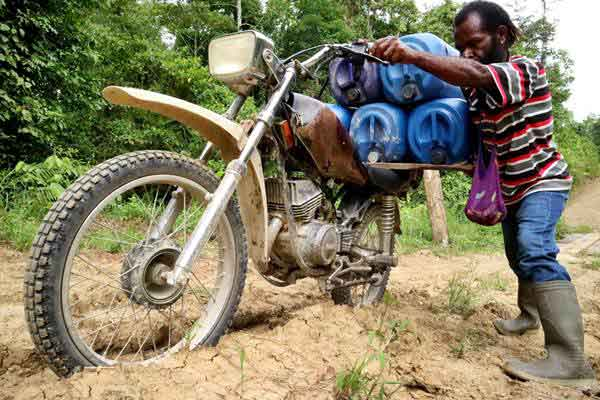
\includegraphics[scale=0.21]
        {Final_Project/image/bbm-papua-221017.jpg}
        \label{f:graph1}
        \end{figure}
    \begin{figure}[t]
        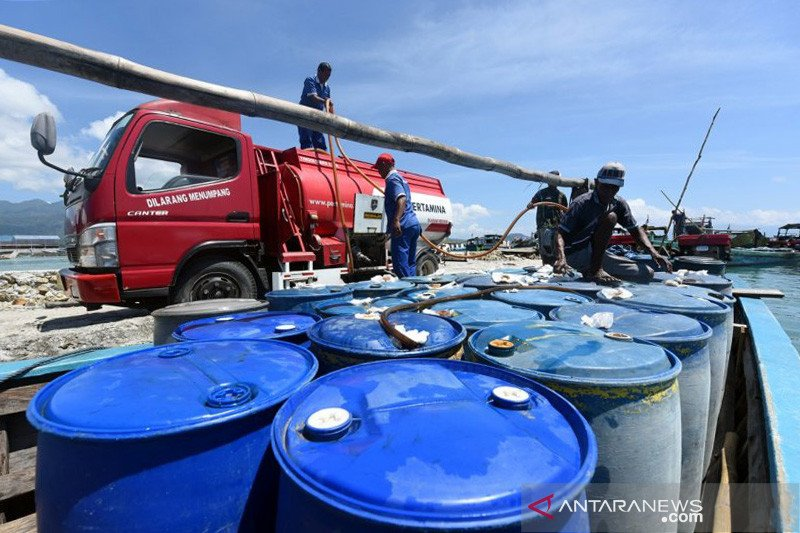
\includegraphics[scale=0.21]
        {Final_Project/image/bbm-satu-harga_1.jpg}
        \label{f:graph2}
        \end{figure}
\end{columns}
\end{frame}

\section{Institutional Context and Conceptual Framework}
\subsection{Accessibility in rural area}
\begin{frame}
\begin{exampleblock}{Transportation Cost}
\begin{itemize}
    \item Transportation spending \al{dominates energy spending} \citep{sambodo_2019}
    \item The \al{lack of adequate and reliable infrastructure} drives up the transportation cost \citep{sandee_2016}.
\end{itemize}
\end{exampleblock}
\end{frame}

\subsection{Fossil fuel subsidy regime}
\begin{frame}
    \begin{columns}[T,onlytextwidth]
    \column{0.33\textwidth}
      \begin{figure}[t]
        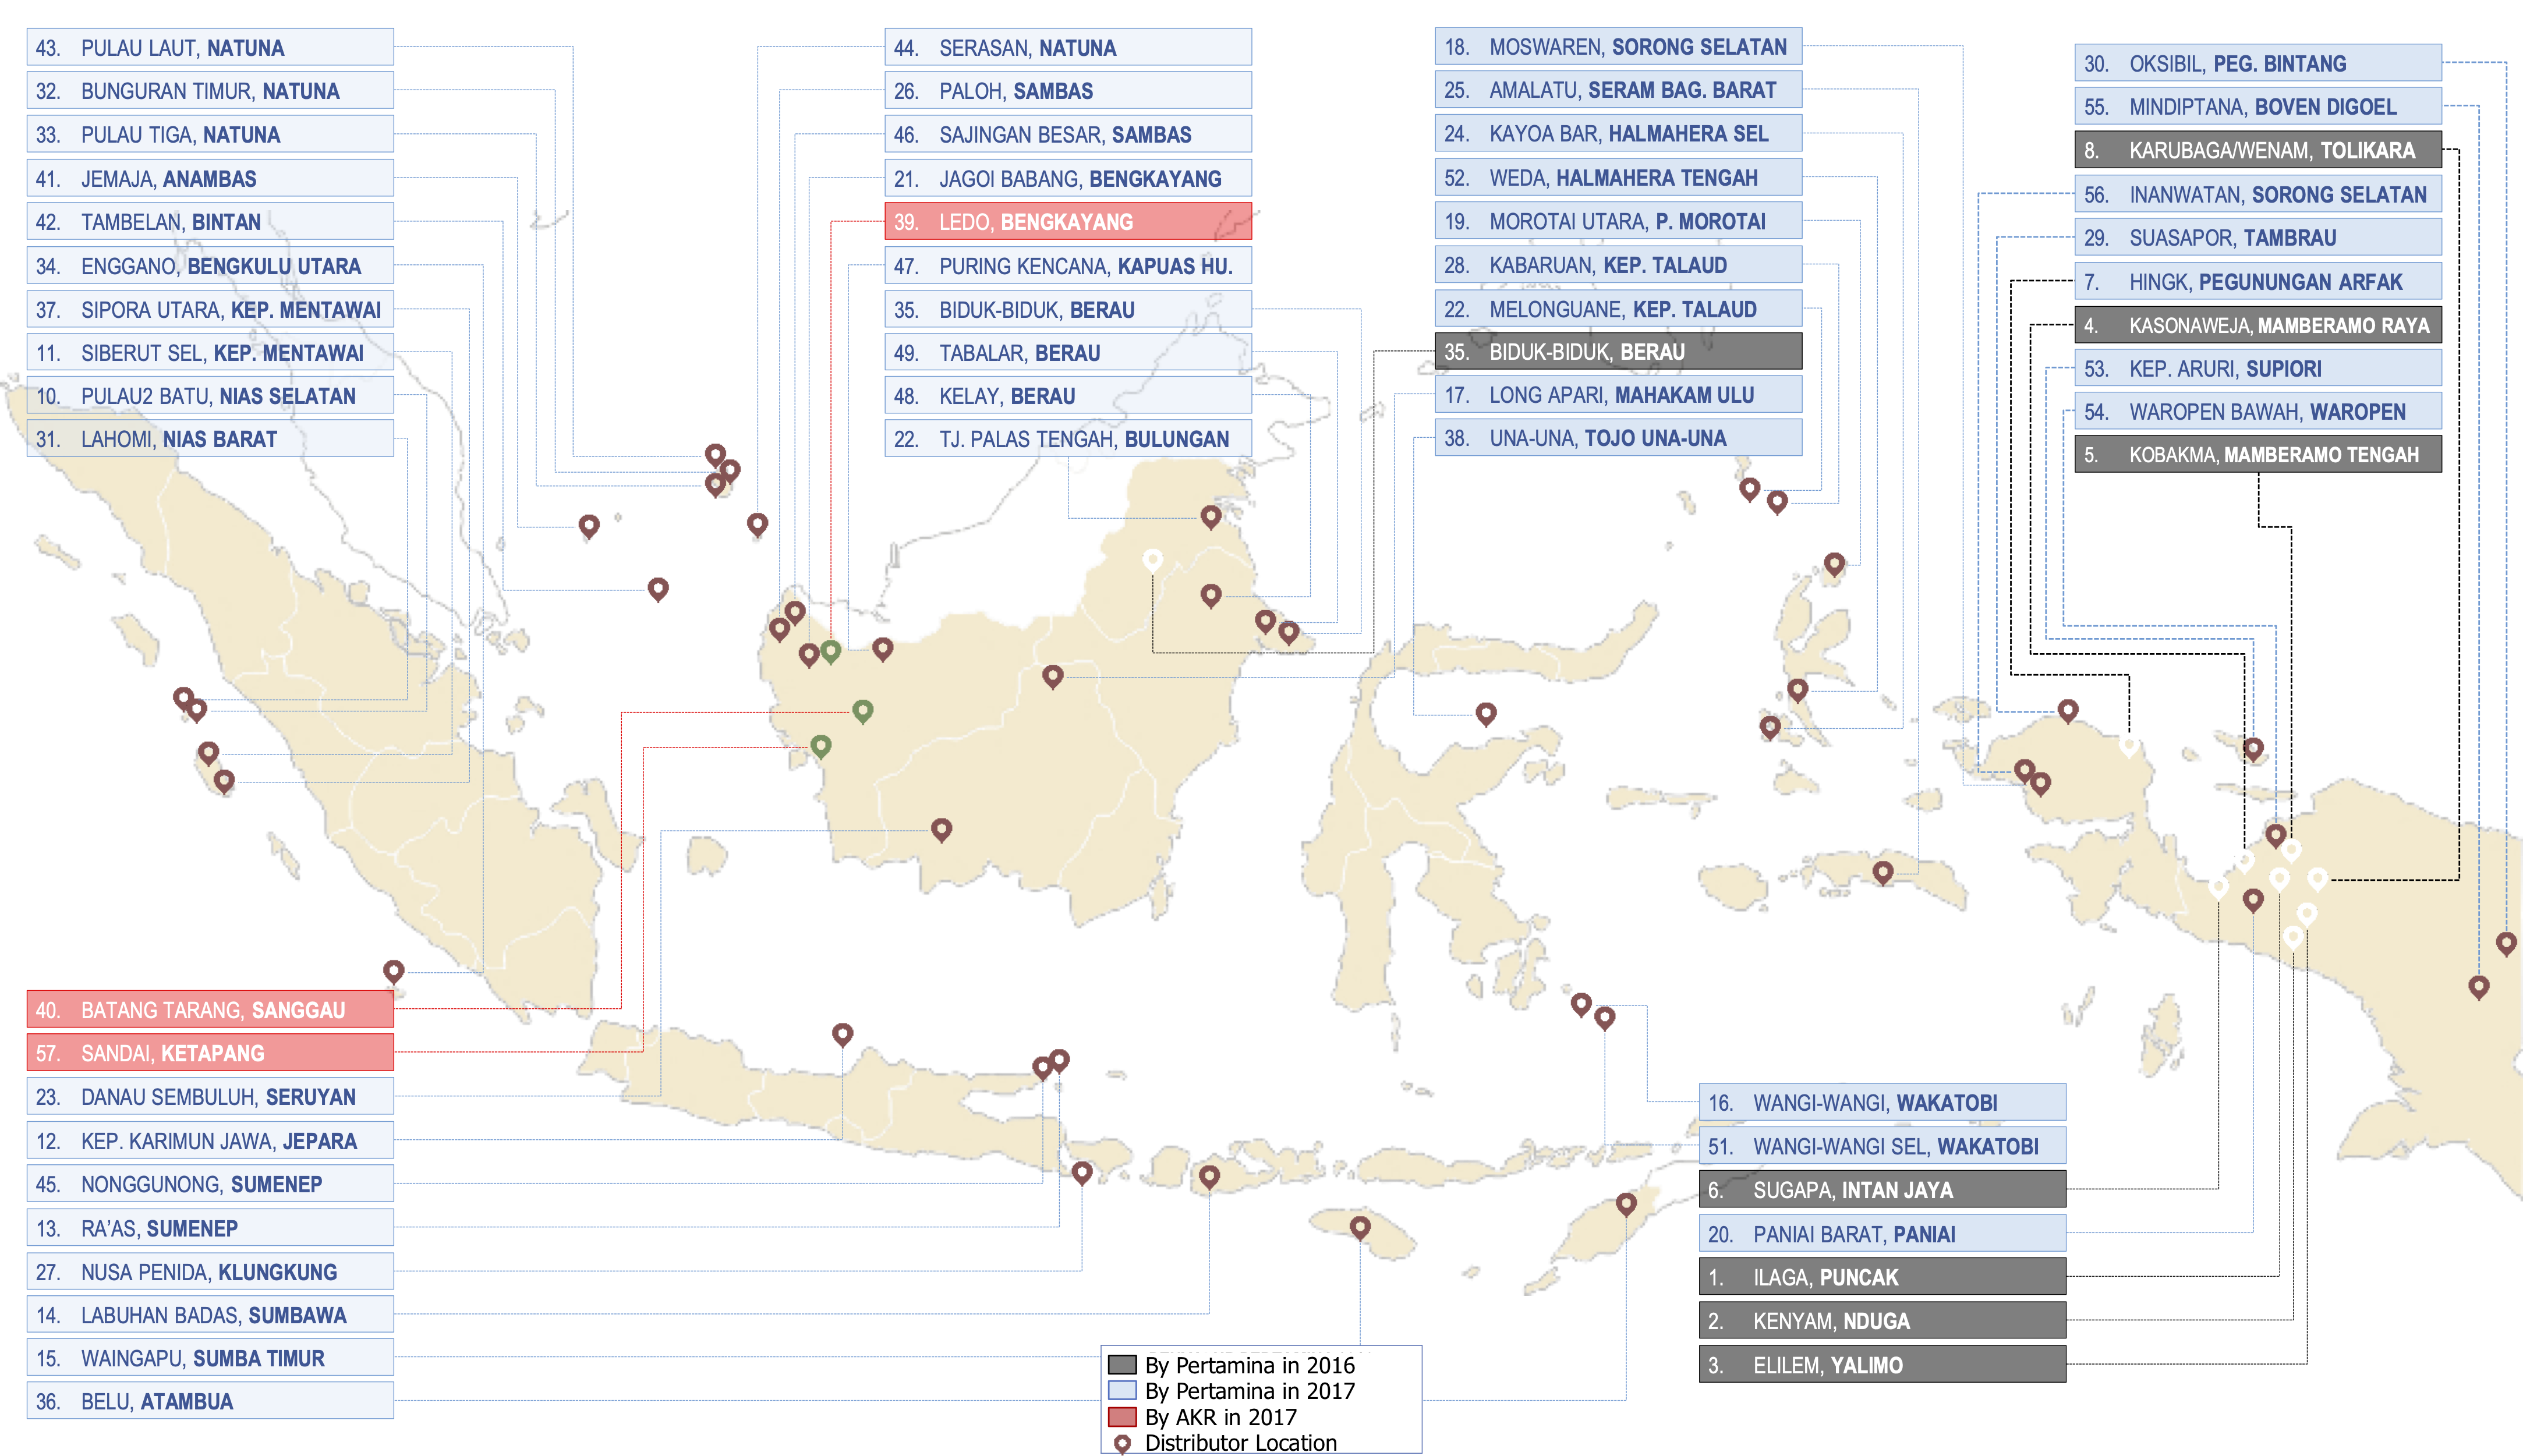
\includegraphics[scale=0.4]{Final_Project/image/BBM Satu Harga.png}
        \caption{New Distributor's Village Location of the Fuel Program}
        \label{f:graph3}
        \end{figure}

    \column{0.67\textwidth}
        \begin{figure}[t]
        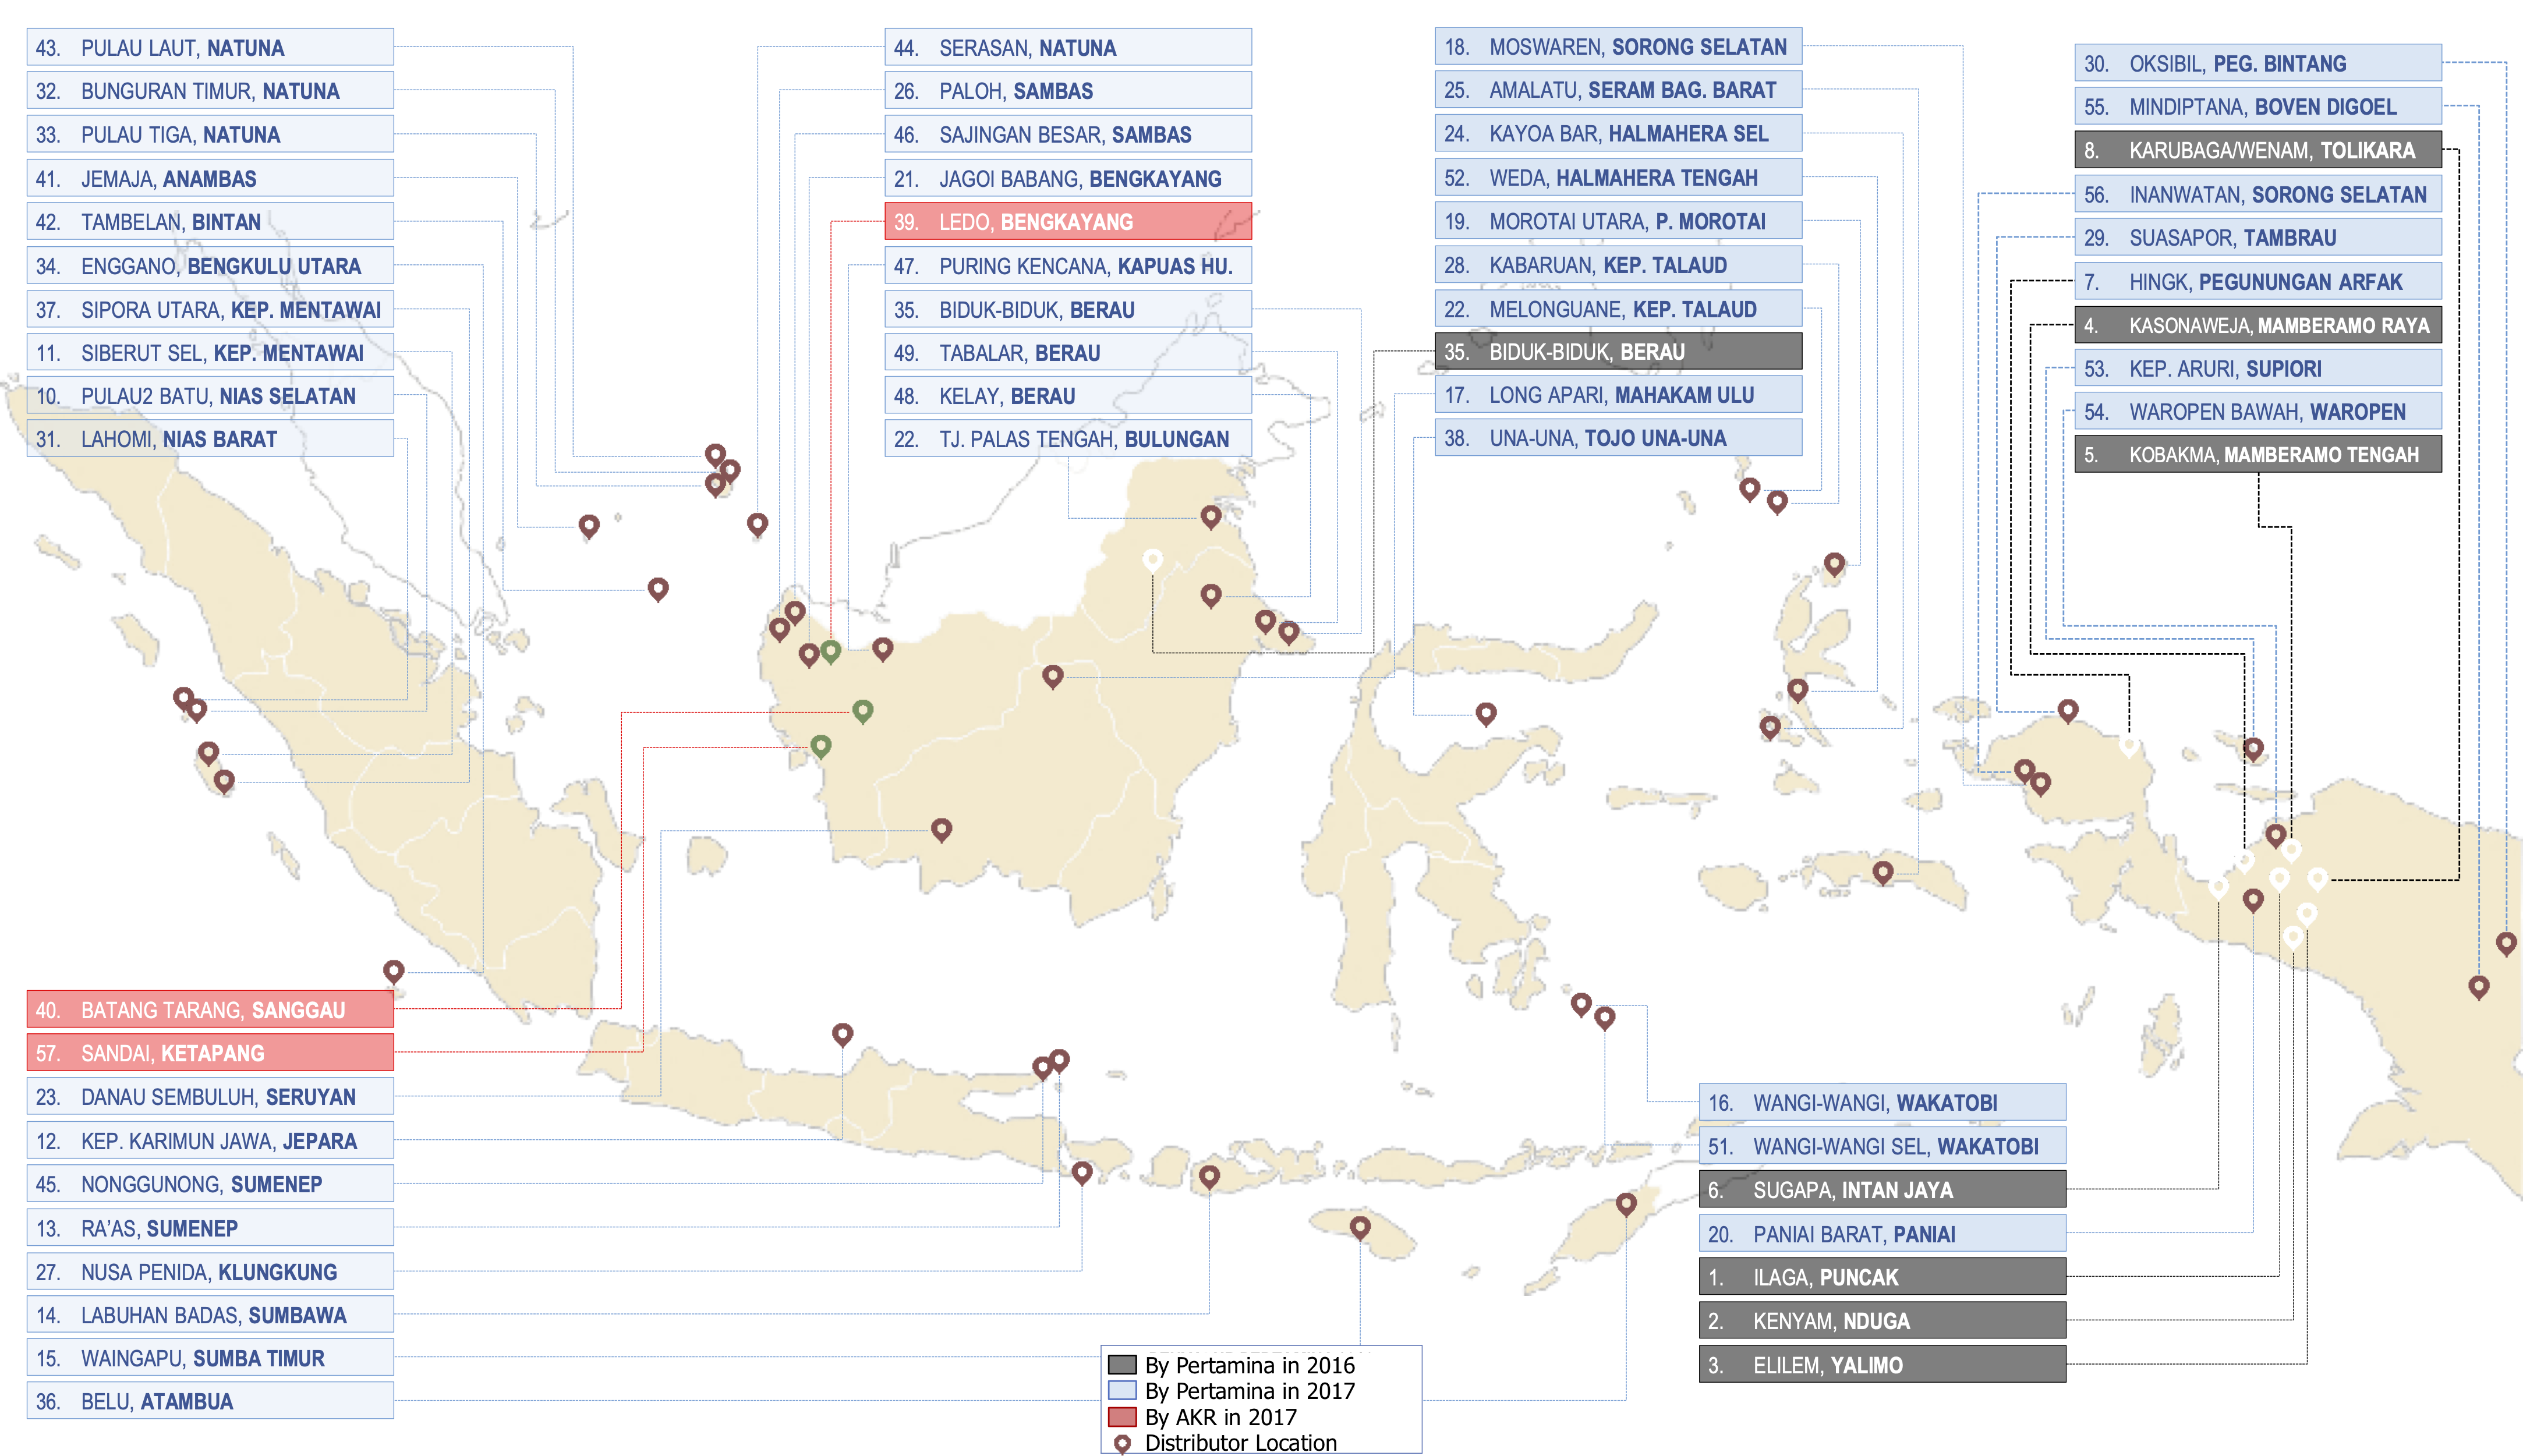
\includegraphics[scale=0.4]{Final_Project/image/BBM Satu Harga.png}
        \caption{New Distributor's Village Location of the Fuel Program}
        \label{f:graph3}
        \end{figure}
    \end{columns}
\end{frame}

\subsection{Decentralization of development}
\begin{frame}
\begin{itemize}
    \item Developing countries believe \alg{decentralization and local government reform} are \alert{\textbf{more efficient}} in bringing local development \citep{vazquez_2017} and \al{providing public goods better} that central government \citep{arends2020}.
    \item 
\end{itemize}
\end{frame}


\begin{frame}
    \begin{figure}[t]
    \subcaptionbox{Village status in 2014\label{f:panel1}}{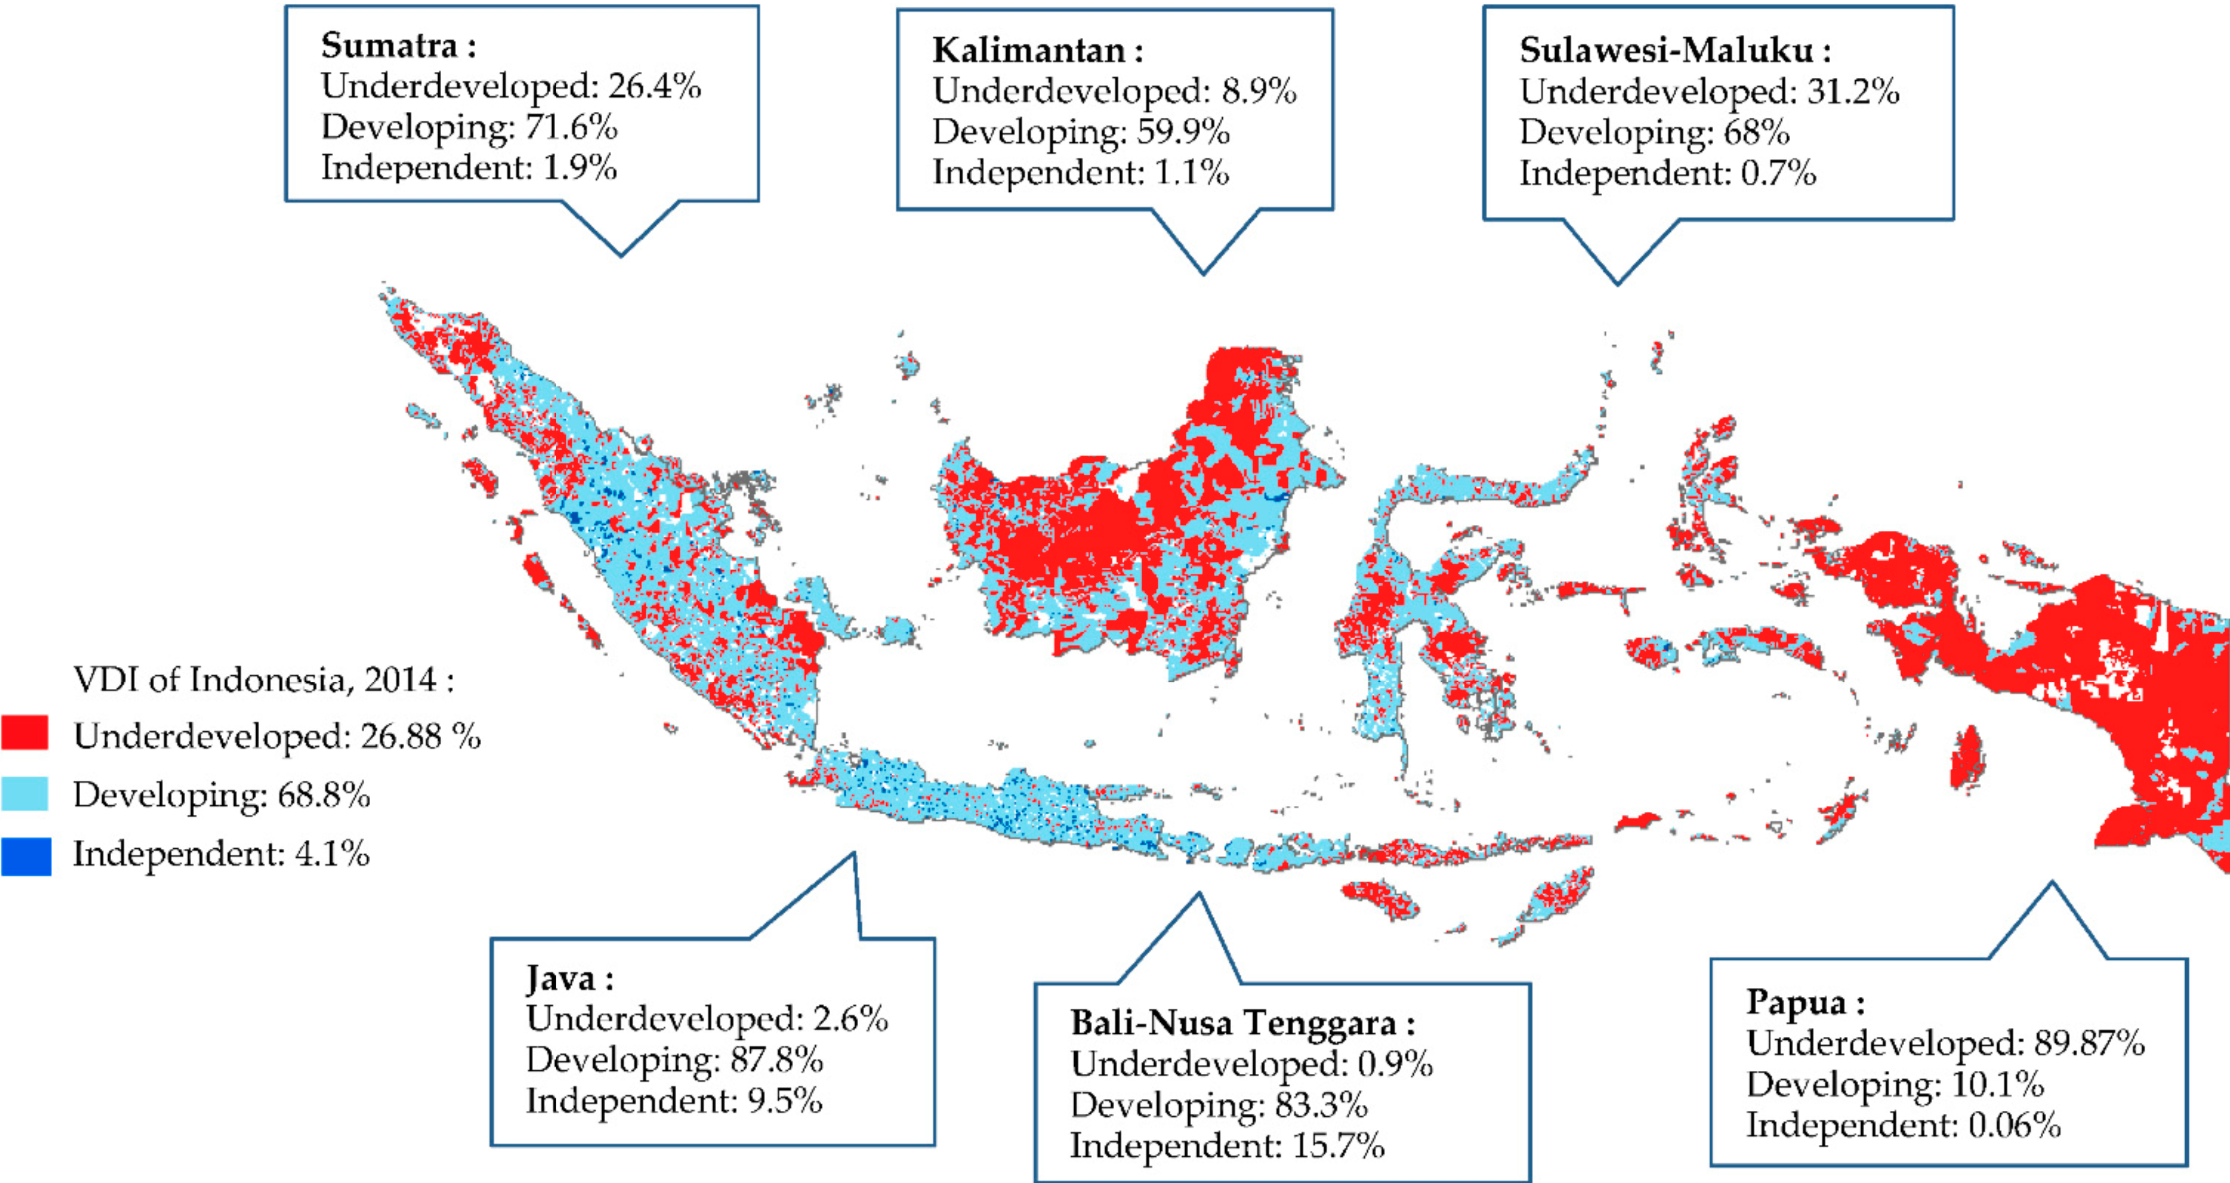
\includegraphics[scale=0.2]{Final_Project/image/vdi2014.png}}\hfill
    \subcaptionbox{Village status in 2018\label{f:panel2}}{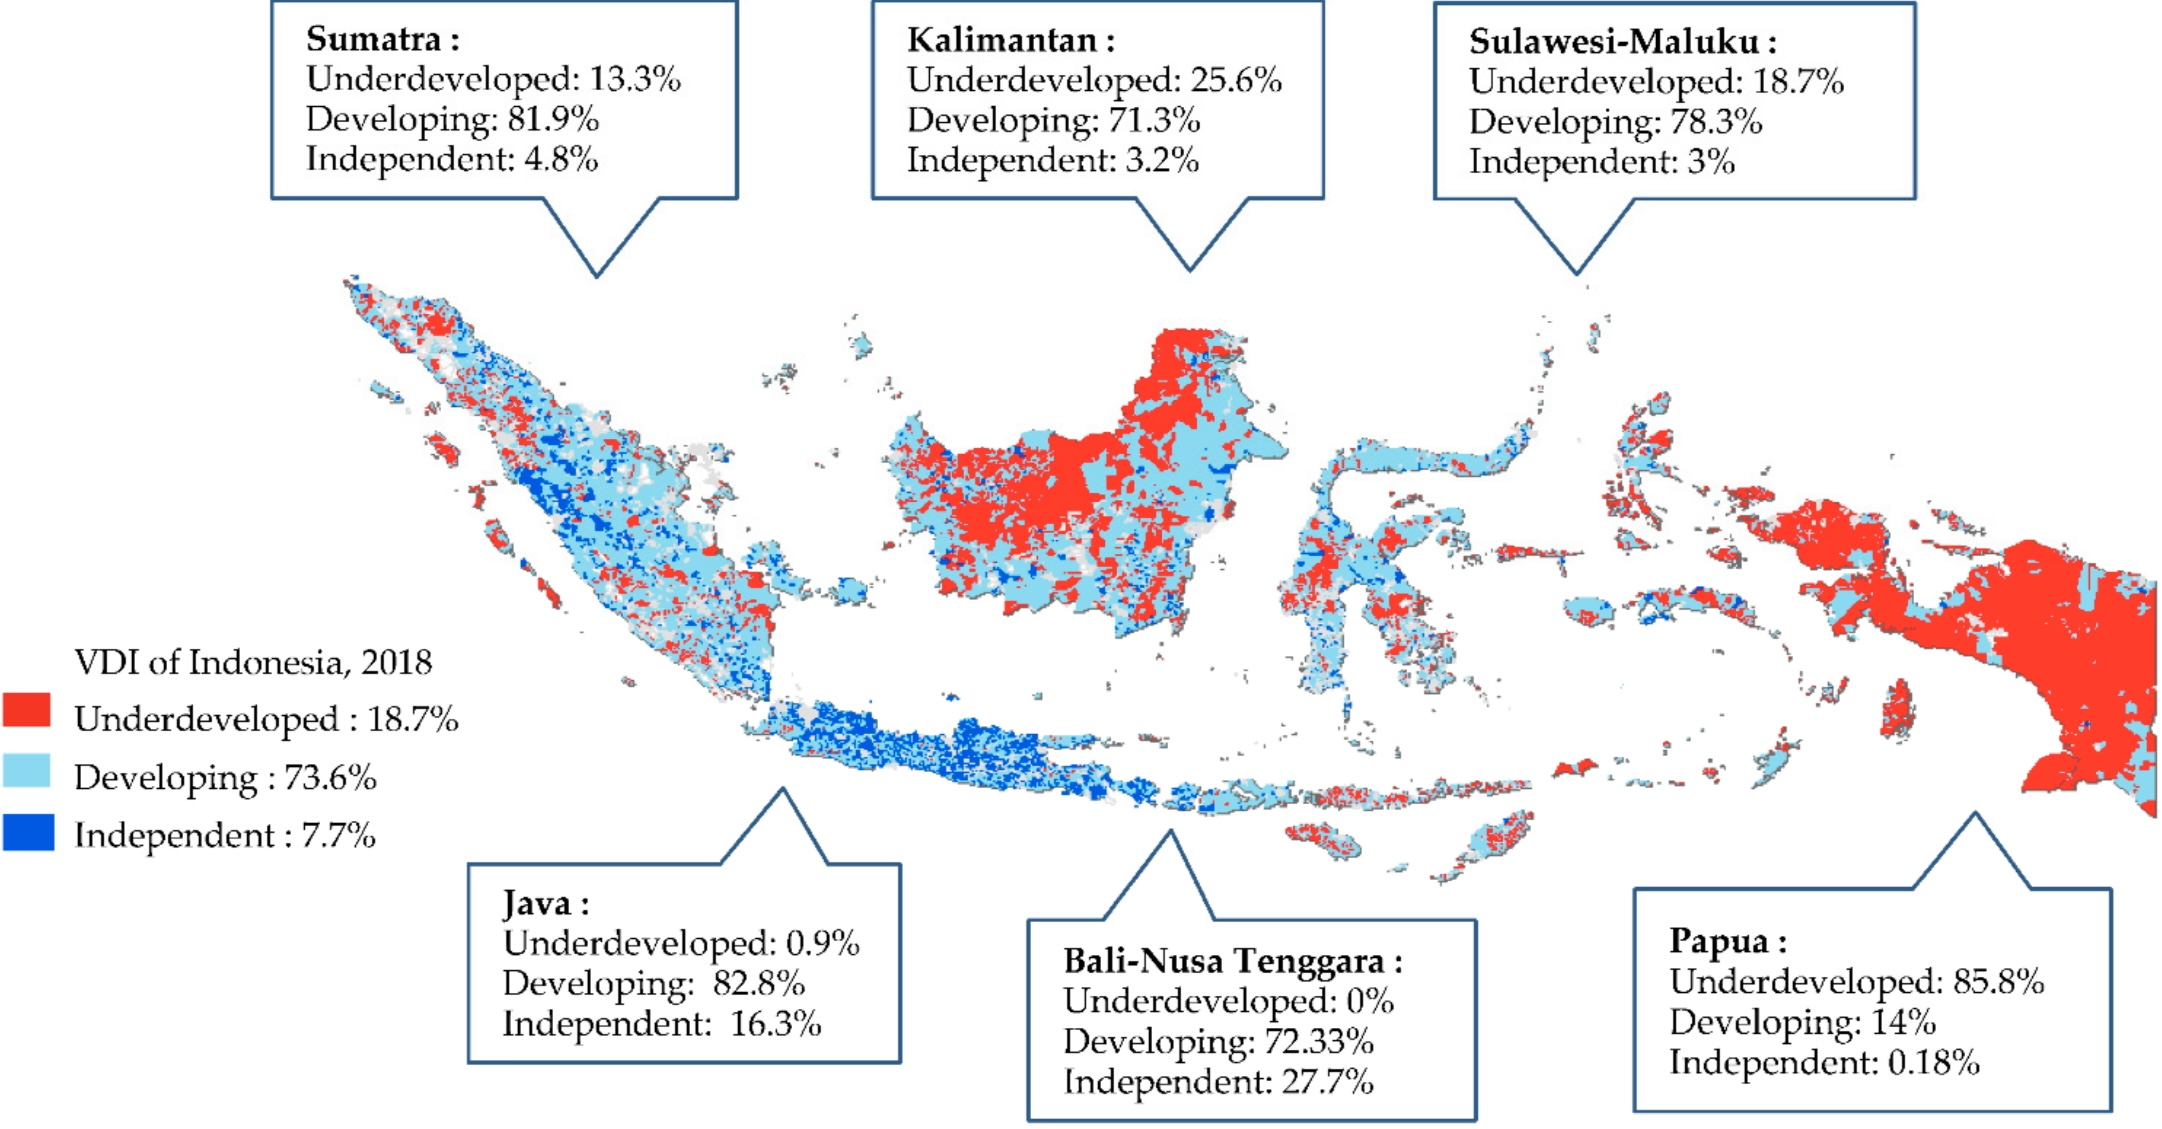
\includegraphics[scale=0.205]{Final_Project/image/vdi2018.jpg}}
    \caption{Indonesia's VDI's status}
    \label{f:graph1}
    \end{figure}
\end{frame}

\section{Data}
\subsection{Data Description}
\begin{frame}
    \begin{itemize}
        \item I obtained the \al{Village Potential Statistics} data for the years 2014 and 2018 from Indonesia's Central Bureau of Statistics complemented with village fund transfer data from the Ministry of Village Development.
        \item I measure rural accessibility using the \al{log of unit transportation cost} (in Rp/km) of each individual village. 
        \footnote{I define unit transportation cost, $y_{it}$, as the \al{transportation cost} from the village office to the sub-district office (in thousands Rp), $c_{it}$, divided by the \al{distance} from the village office to the sub-district office (in km), $d_{it}$.
        \begin{equation}
        y_{it}=\frac{d_{it}}{c_{it}}    
        \end{equation}}
        \item I obtain the list of 57 government-appointed new distributor's village locations from the NOC and then define all the villages that are in the same sub-district as the \al{treated} by the program, i.e. $D_{it}=1$. 
        \begin{itemize}
            \item \alg{For example}, suppose the government in 2016 gives the order for the NOC to build a new distribution point at village $A$. Village $A$ is in the same sub-district as villages $B,C$, and $D$. Then all villages $A,B,C$, and $D$ are treated.
        \end{itemize}
    \end{itemize}
\end{frame}

\subsection{Summary Statistics}
\begin{frame}
    \begin{table}[h]
    \caption{Summary statistics of main variables. }
    \scalebox{0.75}{\begin{tabular}{l*{2}{ccccc}}
\toprule
                &     2014&         &         &         &         &     2018&         &         &         &         \\
                &     Mean&     S.D.&      Min&      Max&     Obs.&     Mean&     S.D.&      Min&      Max&     Obs.\\
\midrule
\emph{Transportation Cost}&         &         &         &         &         &         &         &         &         &         \\
\hspace{0.25cm} Unit transportation cost in 000s Rp./km&     5.14&    21.02&     0.00&  1000.00&     3407&     4.93&    12.47&     0.00&   400.00&     3411\\
\hspace{0.25cm} Travel Duration&     1.27&     1.27&     1.00&    30.00&     3407&     0.74&     2.36&     0.00&    60.50&     3411\\
\vspace{0.05em} \\ \emph{Natural Disaster}&         &         &         &         &         &         &         &         &         &         \\
\hspace{0.25cm} Landfall occurence average per year&     0.07&     0.37&     0.00&     6.00&     3407&     0.10&     0.49&     0.00&     9.00&     3411\\
\hspace{0.25cm} Earthquake occurence average per year&     0.04&     0.35&     0.00&     7.00&     3407&     0.46&     1.60&     0.00&     9.00&     3411\\
\vspace{0.05em} \\ \emph{Infrastructure}&         &         &         &         &         &         &         &         &         &         \\
\hspace{0.25cm} Number of PLN electricity user household&   366.92&   610.20&     0.00&  6726.00&     3407&   422.79&   651.77&     0.00&  6468.00&     3411\\
\hspace{0.25cm} Number of Junior High School&     0.54&     0.85&     0.00&     9.00&     3407&     0.61&     0.89&     0.00&    12.00&     3411\\
\hspace{0.25cm} Number of Senior High School&     0.27&     0.66&     0.00&     7.00&     3407&     0.33&     0.73&     0.00&     8.00&     3411\\
\vspace{0.05em} \\ \emph{Inter-government Transfer}&         &         &         &         &         &         &         &         &         &         \\
\hspace{0.25cm} Revenue from village fund transfer&   113.55&   129.92&     0.00&  1253.00&     3407&   158.93&   289.35&     0.00& 13662.00&     3172\\
\bottomrule
\end{tabular}
}
    \label{t1}\end{table}
\end{frame}

\section{Empirical Strategy}
\subsection{Identification}
\begin{frame}

   \centering
	\begin{minipage}[b]{0.5\textwidth}

	  \begin{block}{Default}
        Block content.
      \end{block}

      \begin{alertblock}{Alert}
        Block content.
      \end{alertblock}

      \begin{exampleblock}{Example}
        Block content.
      \end{exampleblock}      
      
	\end{minipage}	
\end{frame}

\subsection{Model Specification}
\begin{frame}
    \begin{equation*}
        \log(y_{it})=\alpha_i+\delta_1 prog_{it}+\gamma_1 VF_{it}+
    \end{equation*}
\end{frame}


\section{Results}
\subsection{Main Results}
\begin{frame}
    \begin{columns}[T,onlytextwidth]
    \column{0.33\textwidth}
      \textbf{Items}
      \begin{itemize}
        \item Cats 
        \begin{itemize}
            \item British Shorthair
        \end{itemize}
        \item Dogs \item Birds
      \end{itemize}

    \column{0.33\textwidth}
      \textbf{Enumerations}
      \begin{enumerate}
        \item First 
        \begin{enumerate}
            \item First subpoint
        \end{enumerate}
        \item Second \item Last
      \end{enumerate}

    \column{0.33\textwidth}
      \textbf{Descriptions}
      \begin{description}
        \item[Apples] Yes \item[Oranges] No \item[Grappes] No
      \end{description}
\end{columns}
\end{frame}

\subsection{Robustness}
\begin{frame}
    \begin{columns}[T,onlytextwidth]
    \column{0.33\textwidth}
      \textbf{Items}
      \begin{itemize}
        \item Cats 
        \begin{itemize}
            \item British Shorthair
        \end{itemize}
        \item Dogs \item Birds
      \end{itemize}

    \column{0.33\textwidth}
      \textbf{Enumerations}
      \begin{enumerate}
        \item First 
        \begin{enumerate}
            \item First subpoint
        \end{enumerate}
        \item Second \item Last
      \end{enumerate}

    \column{0.33\textwidth}
      \textbf{Descriptions}
      \begin{description}
        \item[Apples] Yes \item[Oranges] No \item[Grappes] No
      \end{description}
\end{columns}
\end{frame}


\section{Concluding Remarks}
\begin{frame}
    \begin{table}
        \caption{Largest cities in the world (source: Wikipedia)}
        \begin{tabular}{@{} lr @{}}
          \toprule
          City & Population\\
          \midrule
          Mexico City & 20,116,842\\
          Shanghai & 19,210,000\\
          Peking & 15,796,450\\
          Istanbul & 14,160,467\\
          \bottomrule
        \end{tabular}
        \hspace*{1cm}
            \setlength\extrarowheight{3pt}
        \begin{tabular}{|lr|}
          \hline
          \rowcolor{primary}\color{white}City & \color{white}Population\\
          \hline
          Mexico City & 20,116,842\\
          Shanghai & 19,210,000\\
          Peking & 15,796,450\\
          Istanbul & 14,160,467\\
          \hline
        \end{tabular}
    \end{table}
\end{frame}

\section{}
\begin{frame}[allowframebreaks]{References}
    \bibliographystyle{Final_Project/paper/bibliography.bst}
    \bibliography{references.bib}
\end{frame}
\end{document}